
El análisis que se hace enfocado en los modelos matemáticos con respecto a la comprensión del suelo es importante, por tanto para mí resulta clave estudiar tesis y trabajos científicos que incursionen en el tema agro, siendo esto indispensable como estudiante de ingeniería agrícola, esto es por tener cierta responsabilidad sobre el cuidado y conocimiento del suelo. Resulta interesante como un estudiante de doctorado llamado Peter bastian presenta sus tesis sobre el análisis matemático computacional en un medio poroso \parencite{Spalding1981} y con sus ideas innova en cierta manera sobre un tema tan imprescindible para las ciencias relacionadas con el suelo. Este trabajo me permite adentrarme significativamente en una solución numérica eficiente de las ecuaciones que rigen el flujo de un fluido en el subsuelo. Es interesante como \parencite{Spalding1981} fusiona de alguna manera métodos numéricos matemáticos los cuales son aplicables en un entorno de medios porosos heterogéneos.\\

Este trabajo proporciona diferentes aclaraciones acerca de cómo se comprende el concepto de \textit{medio poroso}, pues menciona dentro de sus argumentos que es una parte sólida persistente de un compuesto que también se llama matriz sólida, estando entre sus espacios un cuerpo restante llamado espacio poroso el cual se llena con uno o más fluidos, según el autor. Entre los fluidos se encuentran agua, petróleo y gas.\\

Es importante tener en cuenta que para obtener modelos matematicos de fluidos porosos hay que tener presente restricciones como:

\begin{itemize}
	\item El espacio vacío del medio poroso está interconectado.
	\item Las dimensiones del espacio vacío debe ser grandes en comparación con la longitud del camino libre medio de las  moléculas del fluido 
	\item Las dimensiones del espacio vacío deben ser lo suficientemente pequeños como para que el flujo del fluido esté controlado por fuerzas adhesivas en las interfaces fluido-sólido y por fuerzas cohesivas en las interfaces fluido-fluido 
\end{itemize}

De acuerdo con el autor, se comprende que el primer supuesto (P1) es obvio, ya que no puede haber flujo en un espacio vacío desconectado. La segunda propiedad (P2) nos permitirá sustituir las moléculas de fluido en el espacio vacío por un hipotético continuo. Por último, la propiedad (P3) excluye de la definición de medio poroso casos como una red de tuberías.\\

Algo importante a la hora de realizar modelos matemáticos de medios porosos es la consideración de diferentes escalas de longitud, pues en diferentes tipos de suelos se forman secciones transversales que a su vez tienen diferentes escalas siendo las microscópicas en las que se pueden identificar varios tipos de arenas con diferentes tamaños de granos. luego de esta se suele encontrar la regional, es interesante como en la escala microscópica son visibles los granos de arenas individuales y los canales de poros.\\


%\begin{figure}[H]
	%\centering
	%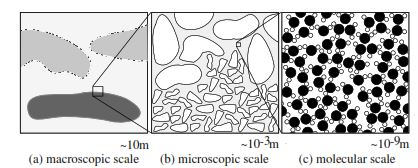
\includegraphics[scale=1]{Imagenes/tipos-de-escalas-peter-bastian}
	%\caption{Diferentes escalas de un medio poroso tomado de la tesis de peter bastian "Numerical Computation of
	%	Multiphase Flows in Porous Media"}
	%\label{escalas-de-medios-porosos.}
%\end{figure}


Peter bastian en su tesis también menciona al realizarse ampliaciones a los suelos a nivel microscópico  se pueden observar espacios vacíos entre sus poros, los cuales pueden llenarse de agua \parencite{Spalding1981}.  Las propiedades de un fluido como la viscosidad, la densidad, el coeficiente de difusión binaria y la miscibilidad, están dadas a escala molecular por propiedades individuales de las moléculas. En la escala microscópica, la configuración del espacio vacío influye en el comportamiento del flujo a través de propiedades como la tortuosidad de los canales de flujo o la distribución del tamaño de los poros, mientras que en la escala macroscópica las inhomogeneidades a gran escala desempeñan un papel importante. Por tanto  el flujo de un fluido newtoniano simple en el espacio vacío de un medio poroso se describe a nivel microscópico mediante el sistema de ecuaciones de Navier-Stokes.





















